\subsection{Show Transport Information about a FixedTask}

If the user wants more information about what kind of vehicles he needs to take to reach others tasks location, he can select a task from the calendar page and automatically more information about that task will be shown. For example, the trip indications and the travel means involved: if he needs to take a bus, a share-based vehicle or his own vehicle. Notice that, if the user take his own private vehicle, the application will schedule the day travels in such a way that allows the user to retake his own vehicle. 

\begin{table}[H]
	\centering
    
    \begin{tabular}{|p{3.5cm}|p{10.3cm}|}
    
    \hline
    \textbf{\large{Actors}}  			& \tabitem User\\
    
    \hline
    \textbf{\large{Goals}} 				& \ref{goal:travel}; \ref{goal:retakeCar}\\
    
    \hline
    \textbf{\large{Enter Condition}}	& The user should be logged in the                                                                    \emph{Travlendar+} system and there is a calendar that is                                         just scheduled\\
    
    \hline
    \textbf{\large{Events Flow}}		& \begin{enumerate}[leftmargin=0.5cm]
                                          	\item The user select a task from his calendar
                                          	\item The user presses the "Show Transport Information" button on the task menu
                                          	\item Now the user can choose from different kind of information: the vehicle he should take, the road trip he should do or the instructions to reach that location
                                          	\item Finally the user can look at the information he needs about transport systems
                                          \end{enumerate}
    										\\
    \hline
    \textbf{\large{Exit Condition}} 	& The user closes the \emph{Transport Information} screen and return to the \emph{Calendar} page\\
    
    \hline
    \textbf{\large{Exception}} 			& \\
    
    \hline
    
    
    \end{tabular}
	
\end{table}

\begin{figure}[H]
\centering
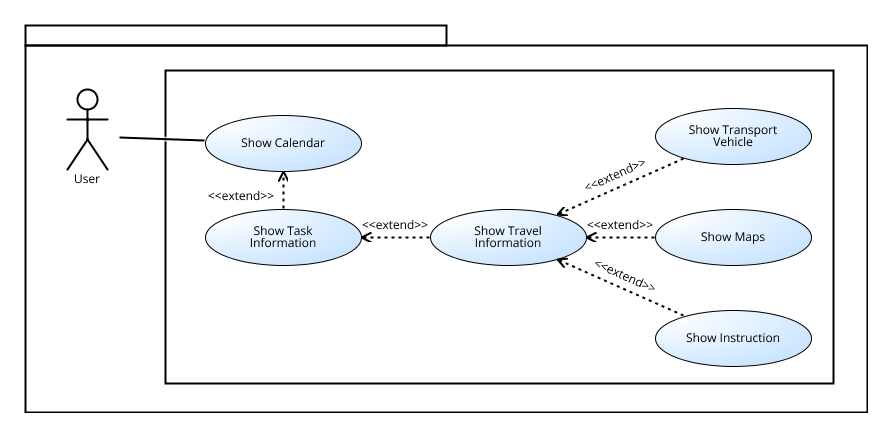
\includegraphics[scale=0.5]{Pictures/UseCaseDiagram/Transport_Instruction.png}
\caption{UML Use Case Diagram for the transport information about a task}
\end{figure}